\documentclass[a4paper]{article}

\usepackage{geometry}

\usepackage[backend=biber,natbib]{biblatex}
\bibliography{library}

\usepackage{clean}
\usepackage{cleveref}
\usepackage{minted}
\setminted{fontsize=\footnotesize,xleftmargin=3em}
\usepackage{subcaption}
\usepackage{tikz}
\usetikzlibrary{calc,positioning}
\tikzset{
	doc/.pic={
		\coordinate (-east)  at (0.309,0);
		\coordinate (-west)  at (-0.309,0);
		\coordinate (-south) at (0,-0.4);
		\coordinate (-north) at (0,0.4);
		\draw[pic actions] (-0.309,-0.4) -- ++(0,0.8) -- ++(0.518,0) -- ++(0,-0.1) -- ++(0.1,0) -- ++(0,-0.7) -- cycle;
		\draw[pic actions] (0.209,0.4) -- ++(0.1,-0.1);
		\draw[pic actions] (-0.209,-0.1) -- ++(0.418,0);
		\draw[pic actions] (-0.209, 0)   -- ++(0.418,0);
		\draw[pic actions] (-0.209, 0.1) -- ++(0.418,0);
	},
	bin/.pic={
		\coordinate (-east)  at (0.309,0);
		\coordinate (-west)  at (-0.309,0);
		\coordinate (-south) at (0,-0.4);
		\coordinate (-north) at (0,0.4);
		\draw[pic actions] (-0.309,-0.4) -- ++(0,0.8) -- ++(0.518,0) -- ++(0,-0.1) -- ++(0.1,0) -- ++(0,-0.7) -- cycle;
		\draw[pic actions] (0.209,0.4) -- ++(0.1,-0.1);
		\node at (0,0.05)  {\scriptsize\texttt{100}};
		\node at (0,-0.2) {\scriptsize\texttt{001}};
	}
}

\title{Cross-Platform Dynamics in Clean\footnote{For brevity, this handout does not contain references. See our previously handed out topic page for details.}}
\author{Camil Staps\footnote{Radboud University Nijmegen} \and Erin van der Veen\footnotemark[2]}

\begin{document}

\maketitle

\section{Dynamics}
In strongly typed languages, it is often useful to be able to box expressions of arbitrary type.
Thus, in the program below the sum of a list of numbers can be computed, ignoring the fact that the numbers have different types:

\begin{minted}{clean}
dynsum :: [Dynamic] -> Maybe Real
dynsum []             = Just 0.0
dynsum [x :: Real:xs] = (+)         x  <$> dynsum xs
dynsum [x :: Int :xs] = (+) (toReal x) <$> dynsum xs
dynsum _              = Nothing

Start = dynsum [dynamic 37, dynamic 5.0]
\end{minted}
%
Dynamics can also contain not fully evaluated expressions.
This is especially useful to store functions or infinite data structures, as in \mintinline{clean}{dynamic [1..]}.
To be able to share dynamics between programs, on 32-bit Windows an interface exists which can dynamically link object code into any application,
	thus allowing programs to share the code of functions needed to evaluate the expression in a dynamic.

A concrete example where dynamics can be useful is Soccer-Fun.\footnote{\url{http://www.cs.ru.nl/P.Achten/SoccerFun/SoccerFun.html}}
Soccer-Fun is an educational project in Clean in which participants write the AI for a simple football team.
Currently, there is no convenient way to play against other teams without sharing your code (which you want to keep secret).
If one would be able to store their team in a dynamic, serialise that dynamic and share it with others,
	a simple interface can be added to the Soccer-Fun GUI to save and load teams as dynamics.

The main issue with this is that teams consist of both data and code and Soccer-Fun can run on multiple platforms.
Therefore we need a way to (un)serialise data and code in a platform-independent manner.

\section{Clean}
In conventional (imperative) programs the state of the program is defined by: the registers, the stack and the heap.
This is not the case in most modern functional programming languages.
In Clean, for example, the state is defined by: the registers, the A-Stack (for references to the graph), the B-Stack (for basic values), the C-Stack (for return addresses) and the graph (comparable to the heap).
Graph rewriting (a more efficient version of term rewriting where the terms are represented as nodes in a graph) is used to reduce the program to it's normal form.
The way the graph must be rewritten is defined in the graph rewriting rules.

When writing a Clean program one is, in essence, providing instructions on how the graph must be rewritten.
As an example, consider the program to compute $4!$ below.
The first three rewriting steps of the program are shown in \cref{fig:rewriting}.

\begin{minted}{clean}
fac :: Int -> Int
fac 0 = 1
fac n = n * fac (n-1)

Start = fac 4
\end{minted}
%
\begin{figure*}[t]
	\small
	\centering
	\begin{subfigure}[b]{.2\linewidth}
		\centering
		\begin{tikzpicture}[clean]
			\node (start) {\texttt{Start}};
		\end{tikzpicture}
		\caption{Initially.}
	\end{subfigure}%
	\begin{subfigure}[b]{.2\linewidth}
		\centering
		\begin{tikzpicture}[clean]
			\node[node args=1] (fac) {\texttt{fac}};
			\node[below=of fac.arg1.south] (4) {\texttt{4}};
			\draw (fac.arg1) -- (4.north);
		\end{tikzpicture}
		\caption{Applying \texttt{Start}.}
	\end{subfigure}%
	\begin{subfigure}[b]{.3\linewidth}
		\centering
		\begin{tikzpicture}[clean]
			\node[node args=2] (times) {\texttt{*}};
			\node[below=of times.arg1.south] (4) {\texttt{4}};
			\node[node args=1,right=of times.arg2.east] (fac) {\texttt{fac}};
			\node[node args=2,right=of fac.arg1.east] (minus) {\texttt{-}};
			\node[right=of minus.arg2.east] (1) {\texttt{1}};
			\draw (times.arg1) -- (4.north);
			\draw (times.arg2) -- (fac.west);
			\draw (fac.arg1) -- (minus.west);
			\draw (minus.arg1) |- (4.east);
			\draw (minus.arg2) -- (1.west);
		\end{tikzpicture}
		\caption{Applying \texttt{fac n}.}
	\end{subfigure}%
	\begin{subfigure}[b]{.2\linewidth}
		\centering
		\begin{tikzpicture}[clean]
			\node[node args=2] (times) {\texttt{*}};
			\node[below=of times.arg1.south] (4) {\texttt{4}};
			\node[node args=1,right=of times.arg2.east] (fac) {\texttt{fac}};
			\node[below=of fac.arg1.south] (3) {\texttt{3}};
			\draw (times.arg1) -- (4.north);
			\draw (times.arg2) -- (fac.west);
			\draw (fac.arg1) -- (3.north);
		\end{tikzpicture}
		\caption{Applying \texttt{-}.}
	\end{subfigure}
	\caption{Rewriting a Clean node\label{fig:rewriting}.}
\end{figure*}
%
When Clean is compiled, the source code is first translated to ABC-code.
ABC-code is a kind of assembly for an abstract machine specialised for graph rewriting.
The fact that the ABC-Machine is an imperative machine ensures that the translation of a functional program to imperative machine code is a relatively small step.
This, in turn, makes it possible for Clean to target many different architectures.

The goal of our study is to be able to share Clean code and data, wrapped in dynamics, between executables on different platforms.
To do this we generate an abstract, platform-independent bytecode from the ABC-code which can be interpreted by the run-time system.
The interpreter has to interwork with native code:
	as an example, consider how the \mintinline{clean}{dynsum} example above is executed when \mintinline{clean}{dynsum} is a native function but the list elements are evaluated by the interpreter.
This oversimplified pipeline is shown in \cref{fig:pipeline}, of which the top line already exists as the standard way to run a Clean program.

The main challenges of this work are:
	a small binary bytecode format;
	an efficient interpreter (or in the future a Just-in-Time compiler);
	an efficient garbage collector;
	looking up the relevant symbols for a Clean expression in the bytecode;
	stripping and linking the bytecode;
	efficient interworking between native code and the interpreter.

\begin{figure*}[b]
	\centering
	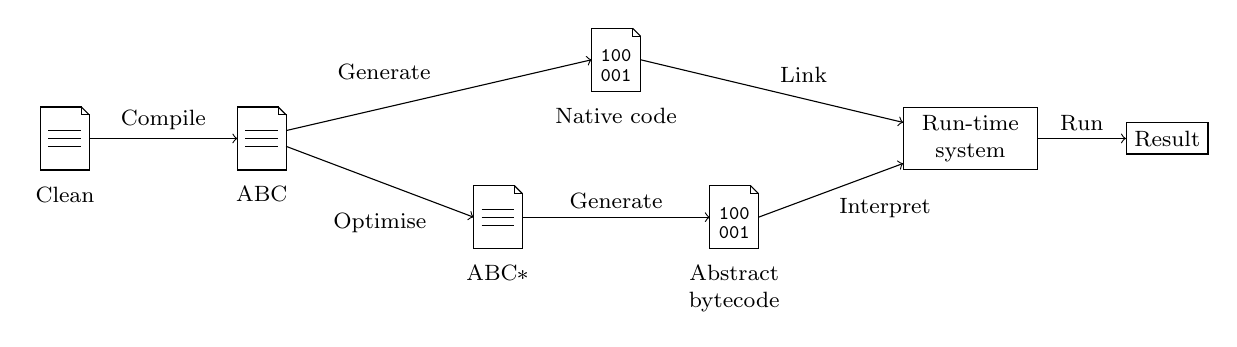
\begin{tikzpicture}
		\footnotesize
		\pic (src) at (-7,0) {doc};
		\node[below=3pt of src-south] {Clean};

		\pic (abc) at (-4.5,0) {doc};
		\node[below=3pt of abc-south] {ABC};
		\draw[->] (src-east) -- node [above] {Compile} (abc-west);

		\pic (pgm) at (0,1) {bin};
		\node[below=3pt of pgm-south] {Native code};
		\draw[->] ($(abc-east)+(0,0.1)$) -- node [left,yshift=1em] {Generate} (pgm-west);

		\pic (opt) at (-1.5,-1) {doc};
		\node[below=3pt of opt-south] {ABC\textasteriskcentered};
		\draw[->] ($(abc-east)-(0,0.1)$) -- node [below,yshift=-1em] {Optimise} (opt-west);

		\pic (bbc) at (1.5,-1) {bin};
		\node[below=3pt of bbc-south,text width=4em,text centered] {Abstract\\bytecode};
		\draw[->] (opt-east) -- node [above] {Generate} (bbc-west);

		\node[draw,text width=5em,text centered] (rts) at (4.5,0) {Run-time\\system};
		\draw[->] (pgm-east) -- node [above right] {Link} (rts);
		\draw[->] (bbc-east) -- node [below right] {Interpret} (rts);

		\node[draw] (res) at (7,0) {Result};
		\draw[->] (rts) -- node [above] {Run} (res);
	\end{tikzpicture}
	\caption{The final pipeline.\label{fig:pipeline}}
\end{figure*}

\printbibliography

\end{document}
